\documentclass[12pt,reqno]{amsart}

\usepackage{amsmath}
\usepackage{amsfonts}
\usepackage{graphicx}
%\usepackage{epstopdf}
\usepackage{hyperref}
\usepackage[left=1in,right=1in,top=0.9in,bottom=0.9in]{geometry}
\usepackage{multirow}
\usepackage{verbatim}
\usepackage{fancyhdr}
\usepackage{mdframed}
\usepackage{natbib}
\renewcommand{\cite}{\citet}

%\usepackage[small,compact]{titlesec} 

%\usepackage{pxfonts}
%\usepackage{isomath}
\usepackage{mathpazo}
%\usepackage{arev} %     (Arev/Vera Sans)
%\usepackage{eulervm} %_   (Euler Math)
%\usepackage{fixmath} %  (Computer Modern)
%\usepackage{hvmath} %_   (HV-Math/Helvetica)
%\usepackage{tmmath} %_   (TM-Math/Times)
%\usepackage{cmbright}
%\usepackage{ccfonts} \usepackage[T1]{fontenc}
%\usepackage[garamond]{mathdesign}
\usepackage{color}
\usepackage[normalem]{ulem}

\newtheorem{theorem}{Theorem}[section]
\newtheorem{conjecture}{Conjecture}[section]
\newtheorem{corollary}{Corollary}[section]
\newtheorem{lemma}{Lemma}[section]
\newtheorem{proposition}{Proposition}[section]
\theoremstyle{definition}
\newtheorem{assumption}{}[section]
%\renewcommand{\theassumption}{C\arabic{assumption}}
\newtheorem{definition}{Definition}[section]

\newtheorem{step}{Step}[section]
\newtheorem{remark}{Comment}[section]
\newtheorem{ex}{Example}[section]
\newtheorem*{ex*}{Example}
\newtheorem{exer}{Exercise}[section]


\newenvironment{example}
  {\begin{mdframed}\begin{ex}}
  {\end{ex}\end{mdframed}}

\newenvironment{exercise}
  {\begin{mdframed}\begin{exer}}
  {\end{exer}\end{mdframed}}

\linespread{1.1}

\pagestyle{fancy}
%\renewcommand{\sectionmark}[1]{\markright{#1}{}}
\fancyhead{}
\fancyfoot{} 
%\fancyhead[LE,LO]{\tiny{\thepage}}
\fancyhead[CE,CO]{\tiny{\rightmark}}
\fancyfoot[C]{\small{\thepage}}
\renewcommand{\headrulewidth}{0pt}
\renewcommand{\footrulewidth}{0pt}

\fancypagestyle{plain}{%
\fancyhf{} % clear all header and footer fields
\fancyfoot[C]{\small{\thepage}} % except the center
\renewcommand{\headrulewidth}{0pt}
\renewcommand{\footrulewidth}{0pt}}

\makeatletter
\renewcommand{\@maketitle}{
  \null 
  \begin{center}%
    \rule{\linewidth}{1pt} 
    {\Large \textbf{\textsc{\@title}}} \par
    {\normalsize \textsc{Paul Schrimpf}} \par
    {\normalsize \textsc{\@date}} \par
    {\small \textsc{University of British Columbia}} \par
    {\small \textsc{Economics 526}} \par
    \rule{\linewidth}{1pt} 
  \end{center}%
  \par \vskip 0.9em
}
\makeatother

\newcommand{\argmax}{\operatornamewithlimits{arg\,max}}
\newcommand{\argmin}{\operatornamewithlimits{arg\,min}}
\def\inprobLOW{\rightarrow_p}
\def\inprobHIGH{\,{\buildrel p \over \rightarrow}\,} 
\def\inprob{\,{\inprobHIGH}\,} 
\def\indist{\,{\buildrel d \over \rightarrow}\,} 
\def\F{\mathbb{F}}
\def\R{\mathbb{R}}
\def\Er{\mathrm{E}}
\def\Pr{\mathrm{P}}
\def\En{\mathbb{E}_n}
\def\Pn{\mathbb{P}_n}
\newcommand{\gmatrix}[1]{\begin{pmatrix} {#1}_{11} & \cdots &
    {#1}_{1n} \\ \vdots & \ddots & \vdots \\ {#1}_{m1} & \cdots &
    {#1}_{mn} \end{pmatrix}}
\newcommand{\iprod}[2]{\left\langle {#1} , {#2} \right\rangle}
\newcommand{\norm}[1]{\left\Vert {#1} \right\Vert}
\newcommand{\abs}[1]{\left\vert {#1} \right\vert}
\renewcommand{\det}{\mathrm{det}}
\newcommand{\rank}{\mathrm{rank}}
\newcommand{\spn}{\mathrm{span}}
\newcommand{\row}{\mathrm{Row}}
\newcommand{\col}{\mathrm{Col}}
\renewcommand{\dim}{\mathrm{dim}}
\newcommand{\prefeq}{\succeq}
\newcommand{\pref}{\succ}
\newcommand{\seq}[1]{\{{#1}_n \}_{n=1}^\infty }
\renewcommand{\to}{{\rightarrow}}
 

\title{Differential Calculus}
\date{\today}

\begin{document}

\maketitle

In this lecture, we will define derivatives for functions on vector
spaces. We will show that all the familiar properties of derivatives
--- the mean value theorem, chain rule, etc --- hold in any vector
space. We will primarily focus on $\R^n$, but we also discuss infinite
dimensional spaces (will we need to differentiate in them to study
optimal control later). All of this material is also covered in
chapter 4 of Carter. Chapter 14 of Simon and Blume and chapter 9 of
Rudin's \textsl{Principles of Mathematical Analysis} cover
differentiation on $\R^n$. Simon and Blume is better for general
understanding and applications, but Rudin is better for proofs and
rigor. 

\section{Derivatives}

\subsection{Partial derivatives}
We have discussed limits of sequences, but perhaps not limits of
functions. To be complete, we define limits as follows.
\begin{definition}
  Let $X$ and $Y$ be metric spaces and $f:X \to Y$.
  \[ \lim_{x \to x_0} f(x) = c \]
  where $x$ and $x_0 \in X$ and $c \in Y$, 
  means that $\forall \epsilon > 0$ $\exists \delta > 0$ such that
  $d(x,x_0) < \delta $ implies $d(f(x),c) < \epsilon$. 
\end{definition}
Equivalently, we could say $ \lim_{x \to x_0} f(x) = c $ means that
for any sequence $\{x_n\}$ with $x_n \to x$, $f(x_n) \to c$. 

You are probably already familiar with the derivative of a function of
one variable. Let $f: \R \to \R$. $f$ is differentiable at $x_0$ if 
\[ \lim_{h \to 0} \frac{f(x_0 + h) - f(x_0)}{h} = \frac{d
  f}{dx}(x_0) \]
exists. Similiarly, if $f: V \to W$ we define its $i$th partial
derivative as follows.
\begin{definition}
  Let $f:\R^n \to R$. The $i$th \textbf{partial derivative} of $f$ is 
  \[ \frac{\partial f}{\partial x_i} (x_0) = \lim_{h \to 0}
  \frac{f(x_{01},...,x_{0i}+h, ... x_{0n}) - f(x_0) }{h}. \]
\end{definition}
The $i$th partial derivative tells you how much the function changes
as its $i$th argument changes.
\begin{example}
  Let $f:\R^n \to \R$ be a production function. Then we call
  $\frac{\partial f}{\partial x_i}$ the \textbf{marginal product} of
  $x_i$. If $f$ is Cobb-Douglas, $f(k,l) = Ak^\alpha l^\beta$, where
  $k$ is capital and $l$ is labor, then the marginal products of
  capital and labor are
  \begin{align*}
    \frac{\partial f}{\partial k} (k,l) = & A \alpha k^{\alpha-1}
    l^\beta \\
    \frac{\partial f}{\partial l} (k,l) = & A \beta k^{\alpha}
    l^{\beta -1}.
  \end{align*}
\end{example}

\subsection{Examples}
\begin{example}
  If $u:\R^n \to \R$ is a utility function, then we call
  $\frac{\partial u}{\partial x_i}$ the marginal utility of $x_i$.  
  If $u$ is CRRA, 
  \[u(c_1,...,c_T) =
  \sum_{t=1}^T \beta^t \frac{c_t^{1-\gamma}}{1-\gamma} \]
  then  the marginal utility of consumption in period $t$ is 
  \[ \frac{\partial u}{\partial c_t} = \beta^t c_t^{-\gamma}. \]
\end{example}

\begin{example}
  The price elasticity of demand is the percentage change in demand
  divided by the percentage change in its price. If $q_1:\R^3 \to \R$ is
  a demand function with three arguments: own price $p_1$, the price
  of another good, $p_2$, and consumer income, $y$.  The own price
  elasticity is 
  \[ \epsilon_{q_1,p_1} = \frac{\partial q_1}{\partial p_1}
  \frac{p_1}{q_1(p_1,p_2,y)}. \]
  The cross price elasticity is the percentage change in demand
  divided by the percentage change in the other good's price, i.e.
  \[ \epsilon_{q_1,p_2} = \frac{\partial q_1}{\partial p_2}
  \frac{p_2}{q_1(p_1,p_2,y)}. \]
  Similarly, the income elasticity of demand is
  \[ \epsilon_{q_1,y} = \frac{\partial q_1}{\partial y}
  \frac{y}{q_1(p_1,p_2,y)}. \]
\end{example}

\subsection{Total derivatives}

Derivatives of univariate functions have a number of useful properties
that partial derivatives do not always share. Examples of useful
properties include univariate derivatives giving the slope of a
tangent line, the implicit function theorem, and Taylor series
approximations. We would like the derivatives of multivariate
functions to have these properties, but partial derivatives are not
enough for this.

\begin{example}\label{ex:nondiff}
  Consider $f:\R^2 \to \R$, 
  \[ f(x,y) = \begin{cases} x^2+y^2 & \text{ if } xy < 0 \\
    x + y \text{ if } xy \geq 0 
  \end{cases}
  \]
  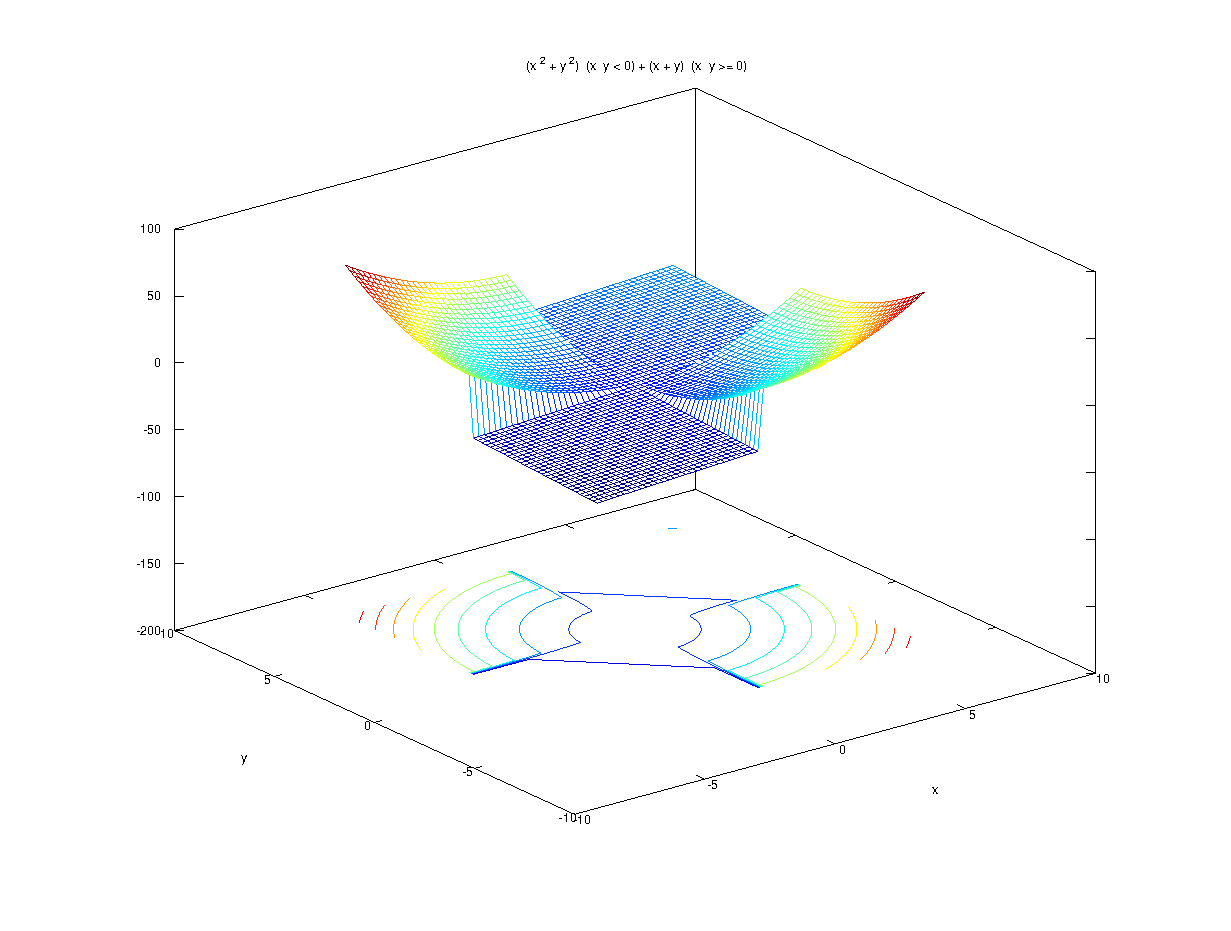
\includegraphics[width=\linewidth]{nondiff}
  
  The partial derivatives of this function at $0$ are $\frac{\partial
    f}{\partial x}(0,0) = 1$ and $\frac{\partial f}{\partial y}(0,0) =
  1$. However, there are points arbitrarily close to zero with
  $\frac{\partial f}{\partial x}(x,y) = 2x + 2y$. If we were to try to
  draw a tangent plane to the function at zero, we would find that we
  cannot. Although the partial derivatives of this function exist
  everywhere, it is in some sense not differentialable at zero (or
  anywhere with $xy = 0$).
\end{example}
Partially motivated by the preceding example, we define the
total derivative (or just the derivative; we're saying ``total'' to
emphasize the difference between partial derivatives and the
derivative).
\begin{definition}
  Let $f: \R^n \to \R$. The \textbf{derivative} (or total derivative
  or differential) of $f$ at $x_0$ is a  linear mapping, $Df_{x_0}:
  \R^n \to \R^1$ such that
  \begin{align*}
    \lim_{h \to 0} \frac{\left|f(x_0 + h) - f(x_0) - Df_{x_0} h\right|} {\norm{h}}
    = 0.
  \end{align*}
\end{definition}
The $h$ in this definition is an $n$ vector in $\R^n$. This is
contrast to the $h$ in the definition of partial derivatives, which
was just a scalar. The fact that $h$ is now a vector is important
because $h$ can approach $0$ along any path. Partial derivatives only
look at the limits as $h$ approaches $0$ along the axes. This allows
partial derivatives to exist for strange functions like the one in
example \ref{ex:nondiff}. We can see that the function from the
example is not differentiable by letting $h$ approach $0$ along a path
that switches from $xy<0$ to $xy\geq 0$ infinitely many times close to
$0$. The limit in the definition of the derivative does not exist
along such a path, so the derivative does not exist. 
\begin{remark}
  In proofs, it will be useful to define $r(x,h) = f(x+h) - f(x) -
  Df_x h$. We will then repeatedly use the fact that $\lim_{h \to 0}
  \frac{|r(x,h)|}{\norm{h}} = 0$.
\end{remark}

If the derivative of $f$ at $x_0$ exists, then so do the partial
derivatives, and the total derivative is simply the $1 \times n$
matrix of partial derivatives.
\begin{theorem}\label{thm:tdiff}
  Let $f: \R^n \to \R$ be differentiable at $x_0$, then
  $\frac{\partial f}{\partial x_i}(x_0)$ exists for each $i$ and 
  \[ Df_{x_0} h = \begin{pmatrix} \frac{ \partial f}{\partial x_1}(x_0) &
    \cdots \frac{ \partial f}{\partial x_n }(x_0)
  \end{pmatrix} h. \]
\end{theorem}
\begin{proof}
  Since $f$ is differentiable at $x_0$, we can make $h = e_i t$ for
  $e_i$ the $i$th standard basis vector, and $t$ a scalar. The
  definition of derivative says that
  \begin{align*}
    \lim_{t \to 0} \frac{\left|f(x_0 + e_i t) - f(x_0) - Df_{x_0} (e_i t)\right|}
    {\norm{e_i t} } & = 0.
  \end{align*}
  Let 
  \begin{align*}
    r_i(x_0,t) = f(x_0 + e_i t) - f(x_0) - t D f_{x_0} e_i 
  \end{align*}
  and note that $\lim_{t \to 0} \frac{|r_i(x_0,t)|}{|t|} =
  0$. Rearranging and dividing by $t$, 
  \begin{align*}
    \frac{f(x_0 + e_i t) - f(x_0)}{t} = D f_{x_0} e_i + \frac{r_i(x_0,t)}{t}
  \end{align*}
  and taking the limit
  \begin{align*}
    \lim_{t \to 0} \frac{f(x_0 + e_i t) - f(x_0)}{t} = D f_{x_0} e_i 
  \end{align*}
  we get the exact same expression as in the definition of the partial
  derivative. Therefore, $\frac{\partial f}{\partial x_i} = D
  f_{x_0}e_i$. Finally, as when we first introduced matrices, we know
  that linear transformation $D f_{x_0}$ must be represented by
  \[ Df_{x_0} h = \begin{pmatrix} \frac{ \partial f}{\partial x_1}(x_0) &
    \cdots \frac{ \partial f}{\partial x_n }(x_0)
  \end{pmatrix} h. \]
\end{proof}
We know from example \ref{ex:nondiff} that the converse of this
theorem is false. The existence of partial derivatives is not enough
for a function to be differentiable. However, if the partial
derivatives exist and are continuous in a neighborhood, then the
function is differentiable. 
\begin{theorem}\label{thm:ptdiff}
  Let $f:\R^n \to \R$ and suppose its partial derivatives exist and
  are continuous in $N_\delta(x_0)$ for some $\delta>0$. Then $f$
  is differentiable at $x_0$ with 
  \[ Df_{x_0}= \begin{pmatrix} \frac{ \partial f}{\partial x_1}(x_0) &
    \cdots \frac{ \partial f}{\partial x_n }(x_0)
  \end{pmatrix}. \]
\end{theorem}
\begin{proof}
  Let $h = (h_1, ..., h_n)$ with $\norm{h}<r$. Notice that
  \begin{align} 
    f(x_0+h) - f(x_0) = & f(x_0 + h_1 e_1) - f(x_0) + f(x_0+h_1 e_1 +
    h_2 e_2) - f(x_0 + h_1 e_1) + ... \\
    & + f(x_0 + h) - f\left(x_0 -
    \sum_{i=1}^{n-1} h_i e_i\right) \\
    &  = \sum_{j=1}^n f\left(x_0 + \sum_{i=1}^j h_i e_i\right) -
    f\left(x_0 + \sum_{i=1}^{j-1} h_i e_i\right). \label{eq:earlier}
  \end{align}
  By the mean value theorem (\ref{thm:mvt}), 
  \[ f\left(x_0 + \sum_{i=1}^j h_i e_i\right) -
  f\left(x_0 + \sum_{i=1}^{j-1} h_i e_i\right) = h_j \frac{\partial f}
  {\partial x_j} (x_0 +  \sum_{i=1}^{j-1} h_i e_i + \bar{h}_je_j) \]
  for some $\bar{h}_j$ between $0$ and $h_j$.  The partial derivatives
  are continuous by assumption, so by making $r$ small enough, we can
  make  
  \[\left| \frac{\partial f}
    {\partial x_j} (x_0 +  \sum_{i=1}^{j-1} h_i e_i + \bar{h}_je_j) -
    \frac{\partial f}{\partial x_j}(x_0) \right| < \epsilon /n, \]
  for any $\epsilon>0$. 
  Combined with equation \ref{eq:earlier} now we have,
  \begin{align} 
    f(x_0+h) - f(x_0) = & \sum_{j=1}^n  h_j \left(\frac{\partial f}{\partial
        x_j} (x_0) + \frac{\epsilon}{n}\right) \\
    \left| f(x_0+h) - f(x_0)  - \sum_{j=1}^n  h_j \frac{\partial f}{\partial
        x_j} (x_0) \right| = & \left| \sum_{j=1}^n h_j \epsilon/n \right|
    \\
    \left| f(x_0+h) - f(x_0)  - Df_{x_0} h \right| \leq & \epsilon
    \norm{h} 
  \end{align}
  Dividing by $\norm{h}$ and taking the limit, 
  \[ \lim_{h \to 0} \frac{\left| f(x_0+h) - f(x_0)  - Df_{x_0} h
    \right|}{\norm{h}} \leq \epsilon.
  \]
  This is true for any $\epsilon>0$, so the limit must be 0. 
\end{proof}
A minor modification of this proof would show the stronger result that
$f:\R^n \to \R$ has a continuous derivative on an open set $U
\subseteq \R^n$ if and only if its partial derivatives are continuous
on $U$. We call such a function \textbf{continuously differentiably}
on $U$ and denote the set of all such function as $C^1(U)$. 

\subsection{Mean value theorem}

The mean value theorem in $\R^1$ says that $f(x+h) - f(x) =
f'(\bar{x}) h$ for some $\bar{x}$ between $x+h$ and $x$. The same
theorem holds for multivariate functions. To prove it, we will need a
couple of intermediate results. 
\begin{theorem}
  Let $f:\R^n \to \R$ be continuous and $K \subset \R^n$ be
  compact. Then $\exists x^* \in K$ such that $f(x^*) \geq f(x)
  \forall x \in K$. 
\end{theorem}
\begin{proof}
  In the last set of notes.
\end{proof}
\begin{definition}
  Let $f: \R^n \to \R$. we say that $f$ has a local maximum at $x$ if
  $\exists \delta > 0$ such that $f(y) \leq f(x)$ for all $y \in
  N_\delta(x)$. 
\end{definition}
Next, we need a result that relates derivatives to maxima. 
\begin{theorem}\label{thm:localmax}
  Let $f: \R^n \to \R$ and suppose $f$ has a local maximum at $x$ and
  is differentiable at $x$. Then $Df_x = 0$. 
\end{theorem}
\begin{proof}
  Choose $\delta$ as in the definition of a local maximum. Since $f$
  is differentiable, we can write
  \[ \frac{f(x+h) - f(x)}{\norm{h}} =\frac{ Df_x h +
    r(x,h)}{\norm{h}} \] where $\lim_{h \to 0}
  \frac{|r(x,h)|}{\norm{h}} = 0$. Let $h = t v$ for some $v \in \R^n$
  with $\norm{v} =1$ and $t \in \R$. If $D f_x v > 0$, then for $t>0$
  small enough, we would have $\frac{f(x+tv) - f(x)}{|t|} = D
  f_x v + \frac{r(x,tv)}{|t|} > D
  f_x v / 2 > 0$ and $f(x+tv)> f(x)$ in contradiction to $x$ being a
  local maximum. Similary, if $D f_v v < 0$ then for $t<0$ and small,
  we would have $\frac{f(x+tv) - f(x)}{|t|} = D
  -f_x v + \frac{r(x,tv)}{|t|} > -D
  f_x v / 2 > 0$ and $f(x+tv)> f(x)$. Thus, it must be that $D f_x v =
  0$ for all $v$, i.e. $D f_x = 0$. 
\end{proof}
Now we can prove the mean value theorem.
\begin{theorem}[mean value]\label{thm:mvt}
  Let $f:\R^n \to \R^1$ be in continuously differentiable on some open
  set $U$ (i.e. $f \in C^1(U)$. Let $x, y
  \in U$ be such that the line connecting $x$ and $y$, $\ell(x,y) =
  \{z\in \R^n: z = \lambda x + (1-\lambda) y, \lambda \in [0,1]\}$, is
  also in $U$. Then there is some $\bar{x} \in \ell(x,y)$ such that
  \[ f(x) - f(y) = Df_{\bar{x}} (x-y). \]
\end{theorem}
\begin{proof}
  Let $z(t) = y + t(x-y)$ for $t \in [0,1]$ (i.e.
  $t=\lambda$). Define
  \[ g(t) = f(y) - f(z(t)) + \left(f(x) - f(y)\right) t \] Note that
  $g(0) = g(1) = 0$. The set $[0,1]$ is closed and bounded, so it is
  compact. It is easy to verify that $g(t)$ is continuously
  differentiable since $f$ is continuously differentiable . Hence, $g$
  must attain its maximum on $[0,1]$, say at $\bar{t}$. If $\bar{t} =
  0$ or $1$, then either $g$ is constant, in which case any $\bar{t}
  \in (0,1)$ is also a maximum, or $g$ must have an interior minimum,
  and we can look at the maximum of $-g$ instead. When $\bar{t}$ is
  not $0$ or $1$, then the previous theorem shows that $g'(\bar{t}) =
  0$. Simple calculation shows that
  \[ g'(\bar{t}) = -Df_{z(\bar{t})} (x-y) +  f(x) - f(y) = 0 \]
  so 
  \[ Df_{\bar{x}}(x-y) = f(x) - f(y) \]
  where $\bar{x} = z(\bar{t})$.
\end{proof}

\subsection{Functions from $\R^n \to \R^m$}

So far we have only looked at functions from $\R^n$ to $\R$. Functions
to $\R^m$ work essentially the same way. 
\begin{definition}
  Let $f: \R^n \to \R^m$. The \textbf{derivative} (or total derivative
  or differential) of $f$ at $x_0$ is a linear mapping, $Df_{x_0}:
  \R^n \to \R^m$ such that
  \begin{align*}
    \lim_{h \to 0} \frac{\left\Vert f(x_0 + h) - f(x_0) - Df_{x_0}
        h\right\Vert} {\norm{h}} = 0. 
  \end{align*}
\end{definition}
Theorems \ref{thm:tdiff} and \ref{thm:ptdiff} sill hold with no
modification. The total derivative of $f$ can be represented by the
$m$ by $n$ matrix of partial derivatives,
\[ Df_{x_0}  = \begin{pmatrix} \frac{\partial f_1}{\partial x_1}(x_0) &
  \cdots & \frac{\partial f_1}{\partial x_n}(x_0) \\
  \vdots & & \vdots \\
  \frac{\partial f_m}{\partial x_1}(x_0) & \cdots & \frac{\partial
    f_m}{\partial x_n}(x_0)  
\end{pmatrix}. \] 
This matrix of partial derivatives is often called
the \textbf{Jacobian} of $f$. 

The mean value theorem \ref{thm:mvt} holds for each of the component
functions of $f:\R^n \to \R^m$. Meaning, that $f$ can be written as
$f(x) = \begin{pmatrix} f_1(x) & \cdots & f_m(x) \end{pmatrix}^T$
where each $f_j:\R^n \to \R$. The mean value theorem is true for each
$f_j$, but the $\bar{x}$'s will typically differ with $j$.
\begin{corollary}[mean value for $\R^n \to \R^m$]\label{thm:mvtm}
  Let $f:\R^n \to \R^m$ be in $C^1(U)$ for some open $U$. Let
  $x, y
  \in U$ be such that the line connecting $x$ and
  $y$, $\ell(x,y) =
  \{z\in \R^n: z = \lambda x + (1-\lambda) y, \lambda \in [0,1]\}$, is
  also in $U$. Then there are $\bar{x}_j \in \ell(x,y)$ such that
  \[ f_j(x) - f_j(y) = D{f_j}_{\bar{x}_j} (x-y) \]
  and
  \[ f(x) - f(y) = \begin{pmatrix} D{f_1}_{\bar{x}_1} \\
    \vdots \\
    D{f_m}_{\bar{x}_m} \end{pmatrix} (x-y). 
  \]  
\end{corollary}
Slightly abusing notation, we might at times write $Df_{\bar{x}}$
instead of $\begin{pmatrix} D{f_1}_{\bar{x}_1} & \cdots &
  D{f_m}_{\bar{x}_m} \end{pmatrix}^T$ with the understanding that we
mean the later.   

\subsection{Chain rule}

For univariate functions, the chain rule says that the derivative of
$f(g(x))$ is $f'(g(x)) g'(x)$. The same is true for multivariate
functions.
\begin{theorem} \label{thm:chain}
  Let $f:\R^n \to \R^m$ and $g: \R^k \to \R^n$. Let $g$ be
  continuously differentiable on some open set $U$ and $f$ be
  continuously differentiable on $g(U)$. Then $h:\R^k \to \R^m$, $h
  (x) = f(g(x))$ 
  is continuously differentiable on $U$ with 
  \[ Dh_x = D f_{g(x)} D g_x \]
\end{theorem}
\begin{proof}
  Let $x \in U$. Consider
  \begin{align*}
    \frac{\norm{ f(g(x+d)) - f(g(x))}} {\norm{d}}.
  \end{align*}
  Since $g$ is differentiable by the mean value theorem, $g(x+d) =
  g(x) + Dg_{\bar{x}(d)} d$, so
  \begin{align*}
    \norm{ f(g(x+d)) - f(g(x))} = &  
    \norm{ f(g(x) + D g_{\bar{x}(d)} d ) - f(g(x))} \\
    \leq & \norm{f(g(x) + D g_x d) - f(g(x))} + \epsilon
  \end{align*}
  where the inequality follows from the the continuity of $D g_x$ and
  $f$, and holds for any $\epsilon >0$. $f$ is differentiable, so
  \[ \lim_{D g_x d \to 0} \frac{\norm{f(g(x) + D g_x d) -
      f(g(x)) - D f_{g(x)} D g_x d}} {\norm{D g_x d}} = 0 \]
  Using the Cauchy-Schwarz inequality, $\norm{D g_x d} \leq \norm{D
    g_x} \norm{d}$, we get
  \[ \frac{\norm{f(g(x) + D g_x d) -
      f(g(x)) - D f_{g(x)} D g_x d}} {\norm{D g_x} \norm{d}} \leq
  \frac{\norm{f(g(x) + D g_x d) -
      f(g(x)) - D f_{g(x)} D g_x d}} {\norm{D g_x d}} 
  \]
  so
  \[ \lim_{ d \to 0} \frac{\norm{f(g(x) + D g_x d) -
      f(g(x)) - D f_{g(x)} D g_x d}} {\norm{d}} = 0. \]   
\end{proof}

\subsection{Higher order derivatives}
We can take higher order derivatives of multivariate functions just
like of univariate functions. If $f: \R^n \to \R^m$, then is has $nm$
partial first derivatives. Each of these has $n$ partial derivatives,
so $f$ has $n^2m$ partial second derivatives, written
$\frac{\partial^2 f_k}{\partial x_i \partial x_j}$. 
\begin{theorem}
  Let $f: \R^n \to \R^m$ be twice continuously differentiable on some
  open set $U$. Then
  \[ \frac{\partial^2 f_k}{\partial x_i \partial
    x_j}(x) =  \frac{\partial^2 f_k}{\partial x_j \partial
    x_i} (x) \]
  for all $i,j,k$ and $ x \in U$.
\end{theorem}
\begin{proof}
  Using the definition of partial derivative, twice, we have
  \begin{align*}
    \frac{\partial^2 f}{\partial x_i \partial x_j} = & \lim_{t_j \to 0}
    \frac{ \lim_{t_i \to 0} \frac{ f(x + t_i e_i + t_j e_j) - f(x +
        t_j e_j)}{t_i} - \lim_{t_i \to 0} \frac{ f(x + t_i e_i) -
        f(x)}{t_i} }{t_j} \\
    = & \lim_{t_j \to 0} \lim_{t_i \to 0} \frac{f(x+t_je_j + t_i e_i)
      - f(x + t_j e_j) - f(x + t_i e_i) + f(x)} {t_j t_i}
  \end{align*}
  from which it is apparent that we get the same expression for $
  \frac{\partial^2 f}{\partial x_j \partial x_i} $.\footnote{This
    proof is not completely correct. We should carefully show that we
    can interchange the order of taking limits. Interchanging limits
    is not always possible, but the assumed continuity makes it
    possible here.}
\end{proof}
The same argument shows that in general the order of partial
derivatives does not matter.
\begin{corollary}
  Let $f: \R^n \to \R^m$ be $k$ times continuously differentiable on
  some open set $U$. Then 
  \[ \frac{\partial^k f}{\partial x_1^{j_1} \cdots
     \partial x_n^{j_n}} = 
  \frac{\partial^k f}{\partial x_{p(1)}^{j_{p(1)}}  \cdots \partial
    x_{p(n)}^{j_{p(n)}}} \]
  where $\sum_{i=1}^n j_i = k$ and $p:\{1,..,n\} \to \{1,...,n\}$ is
  any permutation (i.e. reordering).
\end{corollary}

\subsection{Taylor series}

You have probably seen Taylor series for univariate functions
before. A function can be approximated by a polynomial whose
coefficients are the function's derivatives. 
\begin{theorem}
  Let $f: \R \to \R$ be $k+1$ times continuously differentiable on some
  open set $U$, and let $a$, $a+h \in U$. Then 
  \[ f(a+h) = f(a) + f'(a) h + \frac{f^2(a)}{2} h^2 + ... +
  \frac{f^k(a)}{k!} h^k + \frac{f^{k+1}(\bar{a})}{(k+1)!} h^{k+1}
  \]
  where $\bar{a}$ is between $a$ and $h$. 
\end{theorem}
The same theorem is true for multivariate functions.
\begin{theorem}
  Let $f:\R^n \to \R^m$ be $k$ times continuously differentiable on
  some open set $U$ and $a, a+h \in U$. Then there exists a $k$ times
  continuously differentiable function $r_k(a,h)$ such that
  \[ f(a+h) = f(a) + \sum_{\sum_{i=1}^n {j_i}=1}^k\frac{1}{k!}
  \frac{\partial^{\sum j_i} f}{\partial x_{1}^{j_1} \cdots \partial
    x_{n}^{j_n}}(a) h_1^{j_1}h_2^{j_2} \cdots h_n^{j_n} + r_k(a,h) \]
  and $\lim_{h \to 0} \norm{r_k(a,h)}{\norm{h}^k} = 0$.
\end{theorem}
\begin{proof}
  Follows from the mean value theorem. For $k=1$, the mean value
  theorem says that
  \begin{align*}
    f(a+h) - f(a) = & Df_{\bar{a}} h \\
    f(a+h) = & f(a) + Df_{\bar{a}} h \\
    = & f(a) + Df_{a} h + \underbrace{(Df_{\bar{a}} -Df_a)h}_{r_1(a,h)}  
  \end{align*}
  $Df_a$ is continuous as a function of $a$, and as $h \to 0$,
  $\bar{a} \to a$, so $\lim_{h \to 0} r_1(a,h) = 0$, and the theorem
  is true for $k = 1$. For general $k$, suppose we have proven the
  theorem up to $k-1$. Then repeating the same argument with the
  $k-1$st derivative of $f$ in place of $f$ shows that theorem is true
  for $k$. The only complication is the division by $k!$. To see where
  it comes from, we will just focus on $f:\R \to \R$. The idea is the
  same for $\R^n$, but the notation gets messy. Suppose we want a
  second order approximation to $f$ at $a$, 
  \[ \hat{f}(h) = f(a) + f'(a) h + c_2 f^2(a) h^2 \] and pretend that we
  do not know $c_2$. Consider $f(a+h) = \hat{f}(h)$. Applying the mean value
  theorem to the difference of these functions twice, we have
  \begin{align*}
    f(a+h) - \hat{f}(h) = & f(a)-\underbrace{\hat{f}(0)}_{=f(a)}
    + \left[ f'(a + \bar{h}_1) -
      \underbrace{\hat{f}'(\bar{h}_1)}_{=f'(a)}\right] h \\
    = & f'(a) - \hat{f}'(0) + \left[f^{2}(a+\bar{h}_2) -
      \underbrace{\hat{f}^2(\bar{h}_2)}_{=2c_2 f^2(a)}\right] \bar{h}_1 h \\
    = & f^2(a) (1 - 2c_2) \bar{h}_1 h +
    f^3(a + \bar{h}_3)\bar{h}_2\bar{h_1} h 
  \end{align*}
  if we set $c_2 = \frac{1}{2}$, we can eliminate one term and 
  \[ |f(a+h) - \hat{f}(h) | \leq | \underbrace{f^3(a + \bar{h}_3)
    h^3}_{=r_2(a,h)} |.\]  
  Repeating this sort of argument, we will see that setting $c_k =
  \frac{1}{k!}$ ensures that $\lim_{h \to 0}
  \norm{r_k(a,h)}{\norm{h}^k}  = 0$.
\end{proof}

\begin{example}
  The mean value theorem is used often in econometrics to show
  asymptotic normality. Many estimators can be written as
  \begin{align*}
    \hat{\theta}_n \in \argmin_{\theta \in \Theta} Q^n(\theta) 
  \end{align*}
  where $Q^n(\theta)$ is some objective function that depends on the
  sampled data. Examples include least squares, maximum likelihood and
  the generalized method of moments.  Suppose there is also a
  population version of the objective function, $Q^0(\theta)$ and
  $Q^n(\theta) \inprob Q^0(\theta)$ as $n \to \infty$. There is a true
  value of the parameter, $\theta_0$, that satisfies
  \[ \theta_0 \in \argmin_{\theta \in \Theta} Q^0(\theta). \] 
  For example for OLS, 
  \[ Q^n(\theta) = \frac{1}{n} \sum_{i=1}^n (y_i - x_i \theta)^2 \]
  and
  \[ Q^0(\theta) = \mathrm{E}\left[ (Y - X \theta)^2 \right]. \] If
  $Q^n$ is continuously differentiable\footnote{Essentially the same
    argument works if you expand $Q^0$ instead of $Q^n$. This is
    sometimes necessary because there are some models, like quantile
    regression, where $Q^n$ is not differentiable, but $Q^0$ is
    differentiable.} on $\Theta$ and $\hat{\theta}_n \in
  \mathrm{int}(\Theta)$, then from theorem \ref{thm:localmax},
  \[ DQ^n_{\hat{\theta}_n} = 0 \]
  Applying the mean value theorem, 
  \begin{align*}
    0 = & DQ^n_{\hat{\theta}_n} = DQ^n_{\theta_0} + D^2
    Q^n_{\bar{\theta}}(\hat{\theta}_n - \theta_0 ) \\
    \hat{\theta}_n - \theta_0 = & -\left(D^2 Q^n_{\bar{\theta}}
    \right)^{-1} DQ^n_{\theta_0}.
  \end{align*}
  Typically, some variant of the central limit theorem implies
  $\sqrt{n} DQ^n_{\theta_0} \indist N(0,\Sigma)$. For example for
  OLS,
  \[\sqrt{n} DQ^n_\theta = \frac{1}{\sqrt{n}} \sum_i 2 (y_i - x_i
  \theta ) \theta. \] Also, typically $D^2 Q^n_{\bar{\theta}} \inprob
  D^2 Q^0_{\theta_0}$, so by Slutsky's theorem,\footnote{Part of
    Slutsky's theorem says that if $X_n \indist X$ and $Y_n \inprob
    c$, then $X_n/Y_n \indist X/c$.}
  \[ \sqrt{n} (\hat{\theta}_n - \theta_0 ) = -\left(D^2
    Q^n_{\bar{\theta}} \right)^{-1} \sqrt{n} DQ^n_{\theta_0} \indist
  N\left( 0, \left(D^2 Q^0_{\theta_0} \right)^{-1} \Sigma \left(D^2
      Q^0_{\theta_0} \right)^{-1} \right). \]
\end{example}

\section{Functions on vector spaces}
To analyze infinite dimensional optimization problems, we need to
differentiate functions on infinite dimensional vector spaces. We
already did this when studying optimal control, but we glossed over
the details. Anyway, we can define the derivative of a function
between any two vector spaces as follows. 
\begin{definition}
  Let $f: V \to W$. The Fr\'{e}chet \textbf{derivative} of $f$ at
  $x_0$ is a continuous\footnote{If $V$
    and $W$ are finite dimensional, then all linear functions are
    continuous. In infinite dimensions, there can be discontinuous
    linear functions.} linear mapping, $Df_{x_0}: V \to W$ such that
  \begin{align*}
    \lim_{h \to 0} \frac{\left\Vert f(x_0 + h) - f(x_0) - Df_{x_0}
        h\right\Vert} {\norm{h}} = 0. 
  \end{align*}
\end{definition}
Note that this definition is the same as the definition of total
derivative. 
\begin{example}\label{ex:fre}
  Let $V = \mathcal{L}^\infty(0,1)$ and $W = \R$. Suppose $f$ is given by
  \[ f(x) = \int_0^1 g(x(\tau),(\tau)) d\tau \] 
  for some continuously differentiable function $g:\R^2 \to
  \R$. 
  Then $Df_{x}$ is a linear transformation from $V$ to $\R$. How
  can we calculate $Df_x$? If $V$ were $\R^n$ we would calculate the
  partial derivatives of $f$ and then maybe check that they are
  continuous so that theorem \label{thm:ptdiff} holds. For an infinite
  dimensional space there are infinite partial derivatives, so we
  cannot possibly compute them all. However, we can look at
  directional derivatives. 
\end{example}
\begin{definition}
  Let $f: V \to W$, $v \in V$ and $x \in U \subseteq V$ for some open
  $U$. The \textbf{directional derivative} (or G\^{a}teaux derivative
  when $V$ is infinite dimensional)  in direction $v$ at $x$ is
  \begin{align*}
    df(x;v) = \lim_{\alpha \to 0} \frac{f(x + \alpha v) - f(x)}{\alpha}.
  \end{align*}  
  where $\alpha \in \R$ is a scalar.
\end{definition}
Analogs of theorems \ref{thm:tdiff} and \ref{thm:ptdiff} relates the
G\^{a}teaux derivative to the Fr\'{e}chet derivative.
\begin{lemma}\label{lem:fregat}
  If $f: V \to W$ is Fr\'{e}chet differentiable at $x$, then the
  G\^{a}teaux derivative, $df(x;v)$, exists for all $v \in V$, and
  \[ df(x;v) = Df_x v. \]
\end{lemma}
The proof of theorem \ref{thm:ptdiff} relies on the fact that $\R^n$
is finite dimensional. In fact, in an infinite dimensional space it is
not enough that all the directional derivatives be continuous on an
open set around $x$ for the function to be differentiable at $x$; we
also require the directional derivatives to be linear in $v$. In
finite dimensions we can always create a linear map from the partial
derivatives by arranging the partial derivatives in a matrix. In
infinite dimensions, we cannot do that. 
\begin{lemma}\label{lem:gatfre}
  If $f: V \to W$ has G\^{a}teaux derivatives that are linear in $v$
  and ``continuous'' in $x$ in the sense that $\forall \epsilon>0$
  $\exists \delta > 0$ such that if $\norm{x_1 - x} < \delta$, then
  \begin{align*}
    \sup_{v \in V} \frac{\norm{df(x_1;v) - df(x;v)}}{\norm{v}} < \epsilon
  \end{align*}
  then $f$ is Fr\'{e}chet differentiable with $Df_{x_0} v = df(x;v)$.
\end{lemma}
\begin{remark}
  This continuity in $x$ is actually a very natural definition. If $V$
  and $W$ are normed vector spaces, then the set of all bounded (or
  equivalently continuous) linear transformations is also a normed
  vector space with norm 
  \[ \norm{A} \equiv \sup_{v \in V} \frac{\norm{Av}_W}{\norm{v}_V}. \]
  We are requiring $df(x;v)$ as a function of $x$ to be continuous with 
  respect to this norm. 
\end{remark}
\begin{proof}
  Note that
  \[ f(x+h) - f(x) = \int_0^1 df(x+th,h) dt \]
  by the fundamental theorem of calculus (which we should really
  prove, but do not have time for, so we will take it as given). Then,
  \begin{align*}
    \norm{ f(x+h) - f(x) - df(x;h)} = & \norm{ \int_0^1 df(x+th,h) -
      df(x,h) dt} \\
    \leq & \int_0^1 \norm{df(x+th,h) -df(x,h)} dt
  \end{align*}
  By the definition of $\sup$, 
  \[ \norm{\left(df(x+th;h) - df(x;h) \right)} \leq \sup_{v \in V}
  \frac{\norm{\left(df(x+th;v) - df(x;v)
      \right)}}{\norm{v}}\norm{h}. \] 
  The continuity in $x$ implies for any $\epsilon>0$ $\exists
  \delta > 0$ such that if $\norm{th} < \delta$, then 
  \[ \sup_{v \in V}
  \frac{\norm{\left(df(x+th;v) - df(x;v) \right)}}{\norm{v}} <
  \epsilon. \]
  Thus,
  \[ 
  \norm{ f(x+h) - f(x) - df(x;h)} < \int_0^1 \epsilon \norm{h} dt =
  \epsilon \norm{h}. \]
  In other words, for any $\epsilon>0$ $\exists \delta>0$ such that
  if $\norm{h} < \delta$, then 
  \[ \frac{\norm{f(x+h) - f(x) - df(x;h)}} {\norm{h}} < \epsilon, \]
  and we can conclude that $df(x;h) = Df_x h$. 
\end{proof}
\begin{example*}[Example \ref{ex:fre} continued]
  Motivated by lemmas \ref{lem:fregat} and \ref{lem:gatfre}, we can
  find the Fr\'{e}chet derivative of $f$ by computing its G\^{a}teaux
  derivatives. Let $v \in V$. Remember that both $x$ and $v$ are
  functions in this example. Then,
  \[ f(x+\alpha v) = \int_{0}^1 g(x(\tau) + \alpha v(\tau), \tau)
  d\tau \]
  and
  \begin{align*}
    df(x;v) = & \lim_{\alpha \to 0} \frac{\int_0^1 g(x(\tau) + \alpha
      v(\tau), \tau) d\tau}{\alpha} \\
    = & \int_0^1 \frac{\partial g}{\partial x}(x(\tau),\tau) v(\tau)
    d\tau
  \end{align*}    
  Now, we can either check that these derivatives are linear and
  continuous, or just guess and verify that
  \[ Df_x(v) = \int_0^1 \frac{\partial g}{\partial x}(x(\tau),\tau)
  v(\tau) d\tau. \]
  Note that this expression is linear in $v$ as it must be for it to
  be the derivative. Now, we check that the limit in the definition of
  the derivative is zero,
  \begin{align*}
    \lim_{h \to 0} \frac{\norm{f(x+h) - f(x) - Df_x(h) }}{\norm{h}} & = 
      \lim_{h \to 0} \frac{ \abs{ \int g(x(\tau) + h(\tau), \tau) -
        g(x(\tau),\tau) - \frac{\partial g}{\partial x}(x(\tau),\tau)
        h(\tau) d\tau} } {\norm{h}} \\ 
    & \leq \lim_{h \to 0} \frac{  \int \abs{ g(x(\tau) + h(\tau), \tau) -
        g(x(\tau),\tau) - \frac{\partial g}{\partial x}(x(\tau),\tau)
        h(\tau)} d\tau } {\norm{h}} 
  \end{align*}
  where the inequality follows from the triangle inequality.  To
  simplify, let us assume that $g$ and $\frac{\partial g}{\partial x}$
  are bounded. Then, by the dominated convergence, theorem, we can
  interchange the integral and the limit.\footnote{We have not covered
    the dominated convergence theorem. Unless specifically stated
    otherwise, on homeworks and exams you can assume that
    interchanging limits and integrals is allowed. However, do not
    forget that this is not always allowed. The issue is the order of
    taking limits. Integrals are defined in terms of limits (either
    Riemann sums or integrals of simple functions). It is not
    difficult to come up with examples where $a_{m,n}$ is a doubly
    indexed sequence and $\lim_{m \to \infty} \lim_{n \to \infty}
    a_{m,n} \neq \lim_{n \to \infty} \lim_{m \to \infty} a_{m,n}$.  
  } 
  We then have
  \begin{align*}
    \;\; & \leq  \int \lim_{h \to 0} \frac{ \abs{ g(x(\tau) + h(\tau), \tau) -
        g(x(\tau),\tau) - \frac{\partial g}{\partial x}(x(\tau),\tau)
        h(\tau)} } {\norm{h}} d\tau 
  \end{align*}
  The definition of $\frac{\partial g}{\partial x}$ says that
  \[ \abs{\frac{ g(x(\tau) + h(\tau), \tau) -
      g(x(\tau),\tau) - \frac{\partial g}{\partial x}(x(\tau),\tau)
      h(\tau)}{h(\tau)}} \to 0 \]
  Also $\frac{\abs{h(\tau)}}{\norm{h}} \leq 1$ for all $\tau$ because
  in $\mathcal{L}^\infty(0,1)$, $\norm{h} = \sup_{0 \leq \tau \leq 1}
  \abs{h(\tau)}$. Thus, we can conclude that
  \begin{align*}
    \lim_{h \to 0} & \frac{ \abs{ g(x(\tau) + h(\tau), \tau) -
        g(x(\tau),\tau) - \frac{\partial g}{\partial x}(x(\tau),\tau)
        h(\tau)} } {\norm{h}}
    = \\ 
    & = \lim_{h \to 0} \frac{ \abs{ g(x(\tau) + h(\tau), \tau) -
        g(x(\tau),\tau) - \frac{\partial g}{\partial x}(x(\tau),\tau)
        h(\tau)} } {\abs{h(\tau)}} \frac{\abs{h(\tau)}} {\norm{h}}  
    = 0,
  \end{align*}
  so $f$ is Fr\'{e}chet differentiable at $x$ with derivative $Df_x$. 
\end{example*}

With this definition of the derivative, almost everything that we
proved above for functions from $\R^n \to \R^m$ also holds functions
on Banach spaces. In particular, the chain rule, Taylor's theorem, the
implicit function theorem, and the inverse function theorem hold. The
proofs of these theorems on Banach spaces are essential the same as
above, so we will not go over them. If you find this interesting, you
may want to go through the proofs of all these claims, but it is not
necessary to do so. 

The mean value theorem is slightly more delicate. It still holds for
functions $f:V \to \R^m$, but must be modified when the target space
of $f$ is infinite dimensional. We start with the mean value theorem
for $f:V \to \R$. 
\begin{theorem}[Mean value theorem (onto $\R$) \label{thm:mvtr}]
  Let $f:V \to \R^1$ be in continuously differentiable on some open
  set $U$. Let $x, y \in U$ be such that the line connecting $x$ and
  $y$,
  $\ell(x,y) = \{z\in \R^n: z = \lambda x + (1-\lambda) y, \lambda \in
  [0,1]\}$, is also in $U$. Then there is some $\bar{x} \in \ell(x,y)$
  such that
  \[ f(x) - f(y) = Df_{\bar{x}} (x-y). \]
\end{theorem}
\begin{proof}
  Identical to the proof of \ref{thm:mvt}.
\end{proof}
This result can then be generalized to $f:V \to \R^n$ in the same way
as theorem \ref{thm:mvtm}. 

Now, let's consider a first order Taylor expansion for $f:V \to W$:
\begin{align*}
    f(x+h) - f(x) = & Df_{\bar{x}} h \\
    f(x+h) = & f(x) + Df_{\bar{x}} h \\
    = & f(x) + Df_{x} h + \underbrace{(Df_{\bar{x}} -Df_x)h}_{r_1(x,h)}  
\end{align*}
To show that first order Taylor expansions
have small approximation error, we need to show that
$(Df_{\bar{x}} -Df_x)h$ is uniformly small for all possible $h$. When
$W$ is $\R^1$, there is a single $\bar{x}$. When $W = \R^m$, then
$\bar{x}$ is different for each dimension (as in theorem
\ref{thm:mvtm}). However, this is okay because we just take the
maximum over the finitely many different $\bar{x}$ to get an upper
bound on $\norm{(Df_{\bar{x}} -Df_x)h}$. When $W$ is infinite
dimensional, this argument does not work. Instead, we must use a
result called the Hahn-Banach extension theorem, which is closely
related to the separating hyperplane theorem.
\begin{theorem}[Hahn-Banach theorem \label{thm:hb}]
  Let $V$ be a vector space and $g:V \to \R$ be convex. Let
  $S\subseteq V$ be a linear subspace. Suppose $f_0:
  S \to \R$ is linear and 
  \[ f_0(x) \leq g(x) \] 
  for all $x \in S$. Then $f_0$ can be extended to $f:V \to \R$ such
  that 
  \[ f_0(x) = f(x) \]
  for all $x \in S$ and
  \[ f(x) \leq g(x) \]
  for all $x \in V$.
\end{theorem}
\begin{proof}
  We will apply the separating hyperplane theorem to two sets in $V
  \times \R$. Let 
  \[ A = \{(x,a): a > g(x), x \in V, a \in
    \R\}.\]
  Since $g$ is a convex function, $A$ is a convex set. Let
  \[ B = \{(x,a): a = f_0(x), x \in S, a \in \R \} \]
  Since $f_0$ is linear, $B$ is convex. 
  Clearly $A \cap B = \emptyset$. Also, $\int A \neq \emptyset$
  because $A$ is open, so $\int A = A$ and $A \neq \emptyset$ since
  e.g. $(x, g(x) +1) \in A$. 

  Therefore, by the separating hyperplane theorem,
  $\exists \xi \in (V \times \R)^*$ and $c \in \R$ such that
  \[ \xi z_A > c \geq \xi z_B \]
  for all $z_A \in A$ and $z_B \in B$. $B$ is a linear subspace, so it
  must be that $\xi z_B = 0$ for all $z_B \in B$, so we can take
  $c=0$. 
  
  Note that since $(0,1) \in A$, $\xi(0,1) > 0$. Let $f: V \to \R$ be
  given by $f(x) = -\frac{\xi(x,0)}{\xi(0,1)}$. To conclude, we must
  show that $f(x) = f_0(x) $ for all $x \in S$ and $f(x) \leq g(x)$
  for all $x \in V$.  To show that $f(x) = f_0(x) $, by linearity of
  $\xi$ we have
  \begin{align*}
    \xi(x,y) = & \xi(x,0) + y\xi(0,1) \\
    \frac{\xi(x,y)}{\xi(x,0)} = & -f(x) + y 
  \end{align*}
  If $x \in S$, then $\xi(x,f_0(x)) = 0$, so $f(x) = f_0(x)$ for all
  $x \in S$.
  Similarly for any $y > g(x)$, then $(x,y) \in A$, so
  $\frac{\xi(x,y)}{\xi(x,0)} = -f(x) + y>0$, and $y >
  f(x)$. Therefore, $f(x) \leq g(x)$.
\end{proof}
With this result in hand, we now can now prove the mean value theorem
for arbitrary Banach spaces.
\begin{theorem}[Mean value theorem (onto $\R$) \label{thm:mvtr}]
  Let $f:V \to W$ be in continuously differentiable on some open
  set $U$. Let $x, y \in U$ be such that the line connecting $x$ and
  $y$,
  $\ell(x,y) = \{z\in \R^n: z = \lambda x + (1-\lambda) y, \lambda \in
  [0,1]\}$, is also in $U$. Then there is some $\bar{x} \in \ell(x,y)$
  such that
  \[ \norm{f(x) - f(y)}_W \leq \norm{Df_{\bar{x}} (x-y)}_W \leq
    \norm{Df_{\bar{x}}}_{BL(V,W)} \norm{x-y}_V \]
\end{theorem}
\begin{proof}
  Step 1: use the Hahn Banach theorem to show that $\exists \phi \in
  W^*$ with $\norm{\phi}=1$ and $\norm{f(x) - f(y)} = \phi(f(x) -
  f(y))$. The relevant $f_0$ is $f_0(\alpha(f(x) - f(y))) = \alpha
  \norm{f(x) - f(y)}$. 

  Define $g:[0,1] \to \R$ by $g(t) = \phi(f( t x) - f((1-t) y))$ and
  apply the mean value theorem on $\R$ to get 
  \[ \norm{f(x) - f(y)} = \phi Df_{t^*x + (1-t^*) y)} (x-y) \].
\end{proof}



% \section{First order conditions}

% \subsection{Equality constraints}
% To begin our study of constrained optimization, let's look at a
% maximization problem with equality constraints. 
% \[ \max f(x) \text{ s.t. } h(x) = c \]
% where $f: \R^n \to \R$ and $h: \R^n \to \R^m$. You have probably
% analyzed such a problem graphically when $n=2$ and $m=1$. You draw the
% constraint set and the level curves of the objective function. The
% maximum occurs where the level curves are tangent to the
% constraint. There's a nice picture and discussion of this in chapter
% 18.2 of Simon and Blume.  At the point of tangency, the slopes of the
% level curve and the constraint are equal. By the implicit function
% theorem, these slopes are $-\frac{(\partial f)/(\partial x_1)}
% {(\partial f)/(\partial x_2)}$ and$-\frac{(\partial h)/(\partial x_1)}
% {(\partial h)/(\partial x_2)}$. These slopes are equal at the
% maximizer $x^*$, so
% \begin{align*}
%   \frac{(\partial f)/(\partial x_1) (x^*)}
%   {(\partial f)/(\partial x_2)(x^*)} = & \frac{(\partial h)/(\partial x_1)(x^*)}
%   {(\partial h)/(\partial x_2)(x^*)} \\
%   \frac{(\partial f)/(\partial x_1)(x^*)}
%   {(\partial h)/(\partial x_1)(x^*)} = & \frac{(\partial f)/(\partial x_2)(x^*)}
%   {(\partial h)/(\partial x_2)(x^*)} \equiv \mu
% \end{align*}
% where $\mu$ is defined by the above equality. We can then rewrite the
% equation as
% \begin{align}
%   \frac{\partial f}{\partial x_1} (x^*) - \mu \frac{\partial
%     h}{\partial x_1}(x^*) = & 0 \label{ef1} \\
%   \frac{\partial f}{\partial x_2} (x^*) - \mu \frac{\partial
%     h}{\partial x_2}(x^*) = & 0 \label{ef2}
% \end{align}
% We also know that 
% \begin{align}
%   h(x^*) - c = 0\label{ebc}
% \end{align}
% (\ref{ef1}), (\ref{ef2}), and(\ref{ebc}) give us three equations in
% three unknowns ($x_1*, x_2^*, \mu$).  Note that these three equations
% are the first order conditions for maximizing 
% \[ L(x,\mu) \equiv f(x) - \mu(h(x) - c). \]
% This function is called the \textbf{Lagrangian}. $\mu$ is called a
% \textbf{Lagrange multiplier}. 

% The relationship that we just saw for two dimensional functions is
% always true (under some assumptions). Any local maximizer of
% a constrained optimization problem is a critical point of the
% problem's Lagrangian. One way of seeing this is to take a first order
% expansion of the objective (just like we did in the unconstrained
% case) and the constraints. Suppose $x^*$ is a constrained local
% maximizer. Then for $\Delta$ small enough, $f(x^* + \Delta) \leq
% f(x^*)$ for all $x^*+ \Delta$ that satisfy the constraints. If we
% expand $f(x^*+\Delta)$ around $x^*$ we have
% \begin{align*}
%   f(x^*+\Delta) \approx f(x^*) + Df_{x^*} \Delta \leq & f(x^*) \\
%   Df_{x^*} \Delta \leq & 0 
% \end{align*}
% for all $\Delta$ where $x^* + \Delta$ satisfy the constraints. To describe these
% $\Delta$, let's also take an expansion of the constraints around $x^*$.
% \begin{align*}
%   h(x^* + \Delta) \approx & h(x^*) + Dh_{x^*} \Delta
% \end{align*}
% We know that $h(x^*) = c$, so $h(x^* + \Delta) = c$ if and only if
% $Dh_{x^*} \Delta = 0$. Combining the above two observations, if $x^*$
% is a constrained local maximizer, then for all $\Delta$ with $Dh_{x^*}
% \Delta = 0$ we also have $Df_{x^*} \Delta  = 0$. Another way of
% stating this condition is that the null space of $Dh_{x*}$ is
% contained in the null space of $Df_{x*}$, i.e.
% \[ \mathcal{N}(Dh_{x^*}) \subseteq \mathcal{N}(Df_{x^*}). \] Since the
% row space is the orthogonal complement of the null space\footnote{That
%   is, if $x$ is in the row space and $v$ is the null space then
%   $\iprod{x}{v} = 0$ and the dimension of the row space plus the
%   dimension of the null space is $n$}, this is equivalent to saying
% that the row space of the Jacobian of the constraints contains the row
% space of the derivative of $f$, i.e.\footnote{In case you have
%   forgotten the way that we can show that the row and column spaces of
%   a matrix are orthogonal complements is the following. Let $A$ be an
%   $m \times n$ matrix. First, remember that the dimension of the row
%   space is equal to the rank of $A$, and the dimension of the null
%   space is equal to $n$ minus the rank of $A$. Next, suppose $x \in
%   \mathrm{row}(A)$. Then $x \in \mathrm{col}(A^T)$, so there is some
%   $y$ such that $A^T y = x$. Let $v \in \mathcal{N}(A)$. We want to
%   show that $\iprod{x}{v} = 0$. Using the representation of $x$ as
%   $A^T y$, the definition of the transpose, and the definition of the
%   null space, we have
%   \[ \iprod{x}{v} = \iprod{A^T y}{v} = \iprod{y}{A v} = \iprod{y}{0} =
%   0. \]
% }
% \[ \mathrm{row}(Df_{x^*}) \subseteq \mathrm{row}(Dh_{x^*}). \]
% Since $Df_{x^*}$ is $1 \times n$,  this condition is the same as
% saying $Df_{x^*}$ is in the span of the rows of $Dh_{x^*}$. In other
% words, $Df_{x^*}$ is equal to a linear combination of the rows of
% $Dh_{x^*}$, i.e. 
% \[ Df_{x^*} = \mu^T Dh_{x^*}. \]

% The following theorem formally states this result.
% \begin{theorem}[First order condition for maximization with equality constraints] \label{thm:econ}
%   Let $f:U \to \R$ and $h: U \to \R^m$ be continuously
%   differentiable on $U \subseteq \R^n$. Suppose $x^* \in
%   \mathrm{interior}(U)$ is a local maximizer of $f$ on $U$ subject to 
%   $h(x) = c$. Also assume that $Dh_{x^*}$ has rank $m$. Then there
%   exists $\mu^* \in \R^m$ such that $(x^*, \mu^*)$ is a critical point
%   of the Lagrangian,
%   \[ L(x,\mu) = f(x) - \mu^T (h(x) - c). \]
%   i.e.
%   \begin{align*}
%     \frac{\partial L}{\partial x_i}(x^*,\mu^*) = & \frac{\partial
%       f}{\partial x_i} - {\mu^*}^T \frac{\partial h}{\partial
%       x_i}(x^*) = 0 \\
%     \frac{\partial L}{\partial \mu_j}(x^*,\mu^*) = & h(x^*) -
%     c = 0
%   \end{align*}
%   for $i = 1, ..., n$ and $j=1,...,m$.
% \end{theorem}
% The following proof of the theorem gives a third way of arriving at
% the Lagrangian --- this time by using the implicit function
% theorem. You could also prove the theorem by following similar steps
% as in the discussion preceding it.
% \begin{proof} 
%   Consider the $(m+1)$ system of nonlinear equations
%   \begin{align*}
%   f(x) - f_0 & = 0 \\
%   h(x) - c &=0.
%   \end{align*}
%   We know that $x^*$ satisfies this system of equations with $f_0 = f(x^*)$.
%   By the implicit function theorem, if the $(m+1) \times n$ 
%   matrix 
%   \begin{align}
%     \begin{pmatrix} Df_{x^*} \\ Dh_{x^*} \end{pmatrix} \label{drank}
%   \end{align}
%   has full rank then we could write the first $\min\{m+1,n\}$
%   components of $x$ as a function the other components of $x$, $f_0$,
%   and $c$ in some neighborhood of $x^*$. But then there is some
%   $\epsilon > 0$ and $x'$ in this neighborhood of $x^*$ such that 
%   \begin{align*}
%     f(x') = & f_0 + \epsilon  \\
%     h(x)' = & c
%   \end{align*}
%   which contradicts $x^*$ being a local maximum. Therefore, the rank
%   (\ref{drank}) must be less than $m+1$. Thus, the rows of that matrix
%   are linearly dependent, so there exists $\alpha_j$ not all zero such that 
%   \begin{align*}
%     \alpha_0 Df_{x^*} + \alpha_1 D{h_1}_{x^*}  + \cdots + \alpha_m
%     D{h_n}_{x^*} = 0      
%   \end{align*}
%   Moreover it must be that $\alpha_0 \neq 0$ because otherwise
%   $Dh_{x^*}$ would be singular. Setting $\mu_j = \alpha_j/\alpha_0$
%   gives the conclusion of the theorem.
% \end{proof}
% The assumption that $Dh_{x*}$ is non-singular is needed to make sure
% that we don't divide by zero when defining the Lagrange
% multipliers. This assumption is called the \textbf{non-degenerate
%   constraint qualification}. Imposing it makes stating the theorem
% easier, but similar results can be shown without this condition. 

% \subsection{Inequality constraints}

% Now let's consider an inequality instead of equality constraint. 
% \[ \max_{x \in U} f(x) \text{ s.t. } g(x) \leq b. \] 
% When the constraints binds, i.e.\ $g(x^*) = b$, the situation is exactly the
% same as with an equality constraint. However, the constraint does not
% necessarily bind at a local maximum, so we must allow for that
% possibility.  Let $\lambda$ be the Lagrange multiplier for the above
% problem. If the constraint binds, then
% \[ Df_{x^*} - \lambda^T D g_{x^*} = 0. \] 
% Since $Df_{x^*}^T$ is the
% direction in which $f$ increases most rapidly, it must be that going
% in that direction would violate the constraint. That is, for any
% $\delta > 0$
% \begin{align*} 
%   g_j(x^* + \delta Df_{x^*}^T) > & b_j \\
%   g_j(x^*) + \delta Dg_{j,x^*} Df_{x^*}^T + o(\delta^2) > & b \\
%   Dg_{j,x^*} Df_{x^*}^T > & 0
% \end{align*}
% Multiplying the first order condition by $Df_{x^*}^T$ gives
% \[ Df_{x^*} Df_{x^*}^T = \lambda^T D g_{x^*} D f_{x^*}^T. \] 
% Assuming $Df_{x*} \neq 0$, $Df_{x^*} Df_{x^*}^T$ is positive, and, from the previous set of
% inequalities, each element of $D g_{x^*} D f_{x^*}^T$ is also
% positive. Therefore, it must be that when the constraint binds, each
% $\lambda_j > 0$. If the constraint does not bind, we can use the same
% first order condition with $\lambda=0$. Thus, we have $\lambda \geq 0$
% and equals zero iff $g(x^*) < b$. This situation where one of two
% inequalities binds is called a \textbf{complementary slackness
%   condition}.
% \begin{theorem}[First order condition for maximization with inequality
%   constraints] \label{thm:icon} 
%   Let $f:U \to \R$ and $g: U \to \R^m$ be continuously
%   differentiable on $U \subseteq \R^n$. Suppose $x^* \in
%   \mathrm{interior}(U)$ is a local maximizer of $f$ on $U$ subject to 
%   $g(x) \leq b$. Suppose that the first $k \leq m$ constraints, bind
%   \[ g_j(x^*) = b_j \]
%   for $j = 1 ... k$ and that the Jacobian for these constraints, 
%   \[ \begin{pmatrix} 
%     \frac{\partial g_1}{\partial x_1} &  \cdots &\frac{\partial g_1}{\partial x_n}  \\
%     \vdots & & \vdots \\
%     \frac{\partial g_k}{\partial x_1} &  \cdots &\frac{\partial g_k}{\partial x_n}  
%   \end{pmatrix}
%   \]
%   has rank $k$. Then, there exists
%   $\lambda^* \in \R^m$ such that for
%   \[ L(x,\lambda) = f(x) - \lambda^T (g(x) - b). \]
%   we have
%   \begin{align*}
%     \frac{\partial L}{\partial x_i}(x^*,\lambda^*) = & \frac{\partial
%       f}{\partial x_i} - {\lambda^*}^T \frac{\partial g}{\partial
%       x_i}(x^*) = 0 \\
%     \lambda_j^* \frac{\partial L}{\partial \lambda_j}(x^*,\lambda^*) =
%     & \lambda_j^* \left(g(x^*) - b \right)= 0 \\
%     \lambda_j^* & \geq 0 \\
%     g(x^*) & \leq b
%   \end{align*}
%   for $i = 1, ..., n$ and $j=1,...,m$.
% \end{theorem}
% \begin{proof}
%   By our theorem for maximization with equality constraints
%   (\ref{thm:econ}), there exists $\lambda_1^*, ..., \lambda_k^*$ such
%   that   
%   \begin{align*}
%     \frac{\partial L}{\partial x_i}(x^*,\lambda^*) = & \frac{\partial
%       f}{\partial x_i} - {\lambda^*}^T \frac{\partial g}{\partial
%       x_i}(x^*) = 0 \\
%     \lambda_j^* \frac{\partial L}{\partial \lambda_j}(x^*,\lambda^*) =
%     & \left(g(x^*) - c \right)= 0 \\
%   \end{align*}
%   we can set $\lambda_{k+1}^*,..., \lambda_m^*$ to zero, and satisfy
%   all the equations in the conclusion of the theorem.
  
%   All that remains
%   is to verify that $\lambda_1^*\geq 0, ..., \lambda_k^* \geq0$ . Let
%   $g^k: \R^n \to \R^k$ be the $k$ binding constraints and $b^k$ be
%   $(b_1 \cdots b_k)^T$. We know that 
%   \[ g^k(x^*) = b^k. \]
%   By hypothesis, $Dg^k_{x*}$ has rank $k$. Therefore, we can choose
%   $k$ components of $x$ such that
%   \[ \begin{pmatrix}    \frac{\partial g_1}{\partial x_{i1}} &  \cdots &\frac{\partial g_1}{\partial x_{ik}}  \\
%     \vdots & & \vdots \\
%     \frac{\partial g_k}{\partial x_{i1}} &  \cdots &\frac{\partial g_k}{\partial x_{ik}}  
%   \end{pmatrix} = D_{x^k}g^k 
%   \]
%   is invertible. Let $x^k = (x_{i1} \cdots x_{ik})^T $. By the
%   implicit function theorem, we can solve for $x^k$ as a function of
%   the other components of $x$ and $b$. In particular, we could
%   construct a $\chi:[0,\epsilon) \to \R^{n}$ that is continuously
%   differentiable such that $\chi(0) = x^*$ and
%   \begin{align*}
%     g_1(\chi(t)) = & b_1 - t 
%   \end{align*}
%   and $g_i(\chi(t)) = b_i$ for other $i$. Differentiating,
%   \begin{align*}
%     {Dg_1}_{x^*} \chi'(0) = & -1  \\
%     {Dg_j}_{x^*} \chi'(0) = & 0,
%   \end{align*}
%   Also, $\chi(t)$ satisfies the constraints, so it cannot increase
%   $f(x^*)$, i.e.
%   \begin{align*}
%     0 \geq & \frac{d}{dt} f(\chi(t)) |_{t=1} \\
%     0 \geq & Df_{x^*} \chi'(t)
%   \end{align*}
%   From the Lagrangian first order condition, we also know that 
%   \[ Df_{x^*} - \lambda^k Dg^k_{x^*} = 0 \]
%   we can multiply by $\chi'(t)$ to get
%   \begin{align*} 
%     Df_{x^*}\chi'(t) = & \lambda^k Dg^k_{x^*} \chi'(t) \\
%     Df_{x^*} \chi'(t) = & -\lambda_1  \leq 0.
%   \end{align*}
%   Thus $\lambda_1 \geq 0$. We could redefine $\chi(t)$ using $j=2,
%   ..., k$ in place of $1$ to show that the other $\lambda$'s are
%   positive as well.  
% \end{proof}
% In this proof, there is no difference between a binding
% inequality constraint and an equality constraint, so we can easily
% adapt this theorem to maximization problems with both inequality and
% equality constraints.

% \begin{theorem}[First order condition for maximization with mixed constraints] \label{thm:mcon}
%   Let $f:U \to \R$, $h:U \to \R^l$, and $g: U \to \R^m$ be
%   continuously differentiable on $U \subseteq \R^n$. Suppose $x^* \in 
%   \mathrm{interior}(U)$ is a local maximizer of $f$ on $U$ subject to 
%   $h(x) = c$ and $g(x) \leq b$. Suppose that the first $k \leq m$
%   constraints, bind 
%   \[ g_j(x^*) = b_j \]
%   for $j = 1 ... k$ and that the Jacobian for these constraints along
%   with the equality constraints,
%   \[ \begin{pmatrix} 
%     \frac{\partial h_1}{\partial x_1} &  \cdots &\frac{\partial
%       h_1}{\partial x_n}  \\
%     \vdots & & \vdots \\
%     \frac{\partial h_l}{\partial x_1} &  \cdots &\frac{\partial
%       h_l}{\partial x_n}  \\    
%     \frac{\partial g_1}{\partial x_1} &  \cdots &\frac{\partial g_1}{\partial x_n}  \\
%     \vdots & & \vdots \\
%     \frac{\partial g_k}{\partial x_1} &  \cdots &\frac{\partial
%       g_k}{\partial x_n}  
%   \end{pmatrix}
%   \]
%   has rank $k+l$. Then, there exists
%   $\mu^* \in \R^l$ and $\lambda^* \in \R^m$ such that for 
%   \[ L(x,\lambda,\mu) = f(x) - \lambda^T (g(x) - b) - \mu^T(h(x) - c). \]
%   we have
%   \begin{align*}
%     \frac{\partial L}{\partial x_i}(x^*,\lambda^*) = & \frac{\partial
%       f}{\partial x_i} - {\lambda^*}^T \frac{\partial g}{\partial
%       x_i}(x^*) - {\mu^*}^T \frac{\partial h}{\partial x_i}(x^*)= 0 \\
%     \frac{\partial L}{\partial \mu_\ell}(x^*,\lambda^*) = & h_\ell(x^*) - c = 0 \\
%     \lambda_j^* \frac{\partial L}{\partial \lambda_j}(x^*,\lambda^*) =
%     & \lambda_j^* \left(g(x^*) - c \right)= 0 \\
%     \lambda_j^* & \geq 0 \\
%     g(x^*) & \leq b
%   \end{align*}
%   for $i = 1, ..., n$, $\ell = 1,..., l$, and $j=1,...,m$.
% \end{theorem}
% The condition that there are $k$ binding inequality constraints and
% their Jacobian has rank $k$ is another constraint qualification
% condition. This condition occasionally fails to hold, but the
% conclusion of the theorem remains true. There are a number of
% alternative more general constraint qualification conditions. Slater's
% condition is perhaps the most common. Abadie's constraint
% qualification is more general but difficult to check. Chapter 5 of
% Carter has a detailed discussion of other constraint qualification
% conditions.


\section{Optimization in vector spaces}

Recall from earlier that there are many sets of functions that are
vector spaces. We talked a little bit about $\mathcal{L}^p$ spaces of
functions. The set of all continuous functions and the sets of all $k$
times continuously differentiable functions are also vector
spaces. One of these vector spaces of functions will be appropriate
for finding the solution to optimal control problems. Exactly which
vector space is a slightly technical problem dependent question, so we
will not worry about that for now (and we may not worry about it at
all). Similarly, there are vector spaces of infinite sequences. Little
$\ell^p$ is similar to big $\mathcal{L}^p$, but with sequences instead
of functions
\[ \ell^p = \{\{x_t\}_{t=1}^\infty:
\left(\sum_{t=1}^\infty |x_t|^p\right)^{1/p} < \infty\} \]
There are others as well. Again, the right choice of vector space
depends on the problem being considered, and we will not worry about
it too much. 

Given two Banach spaces (complete normed vector spaces), $V$ and $W$,
let $BL(V,W)$ denote the set of all linear transformations from $V$ to
$W$. The derivative of $f:V \to W$ will be in $BL(V,W)$. We can show
that $BL(V,W)$ is a vector space, and we can define a norm on
$BL(V,W)$ by
\[ \norm{D}_{BL(V,W)} = \sup_{\norm{v}_V=1} \norm{D v}_{W} \]
where $\norm{\cdot}_V$ is the norm on $V$ and $\norm{\cdot}_W$ is the
norm on $W$. Moreover, we could show that $BL(V,W)$ is complete. Thus,
$BL(V,W)$ is also a Banach space. Viewed as function of $x$, $Df_x$ is
a function from $V$ to $BL(V,W)$. As we just said, there are both
Banach spaces, so can differentiate $Df_x$ with respect to $x$. In 
this way, we can define the second and higher derivatives of $f:V \to
W$. 

In the previous section we saw that differentiation for functions on
Banach spaces is the same as for functions on finite dimensional
vector spaces. All of our proofs of first and second order conditions
only relied on Taylor expansions and some properties of linear
transformations. Taylor expansions and linear transformations are the
same on Banach spaces as on finite dimensional vector spaces, so our
results for optimization will still hold. Let's just state for the
first order condition for equality constraints. The other results are
similar, but stating them gets to be slightly cumbersome.
\begin{theorem}[First order condition for maximization with equality
  constraints] \label{thm:econv} Let $f:U \to \R$ and $h:U \to W$ be
  continuously differentiable on $U \subseteq V$, where 
  $V$ and $W$ are Banach spaces.  Suppose $x^* \in
  \mathrm{interior}(U)$ is a 
  local maximizer of $f$ on $U$ subject to
  $h(x) = 0$. Suppose that $Dh_{x^*}:V \to W$ is onto. 
. Then, there exists
  $\mu^* \in BL(W,\R)$ such that for
  \[ L(x,\mu) = f(x) - \mu h(x). \]
  we have
  \begin{align*}
     D_xL(x^*,\mu^*) = & Df_{x*} - \mu Dh_{x^*} = 0_{BL(V,\R)} \\
     D_\mu L(x^*,\mu^*) = & h(x^*) = 0_{W}
  \end{align*}
\end{theorem}
There are a few differences compared to the finite dimensional case
that are worth commenting on. First, in the finite dimensional case,
we had $h:U \to \R^m$, and the condition that $\rank Dh_{x^*} =
m$. This is the same as 
saying that the $Dh_{x^*}:\R^n \to \R^m$ is
onto. Rank is not well-defined in infinite dimension, so we now state
this condition as $Dh_{x^*}$ being onto instead of being rank
$m$. 

Secondly, previously $\mu \in \R^m$, and the Lagrangian was 
\[ L(x,\mu) = f(x) - \mu^T h(x). \] Viewed as a $1$ by $m$ matrix,
$\mu^T$ is a linear transformation from $\R^m$ to $\R$. Thus, in the
abstract case, we just say $\mu \in BL(W,\R)$, which as when we defined
transposes, is called the dual space of $W$ and is denoted $W^\ast$.

Finally, we have subscripted the zeroes in the first order condition
with $BL(V,\R)$ and $W$ to emphasize that the first equation is for
linear transformations from $V$ to $\R$, and the second equation is in
$W$. $Df_{x*}$ is a linear transformation from $V$ to
$\R$. $Dh_{x*}$ goes from $V$ to $W$. $\mu$ goes from $W$ to $\R$, so
$\mu$ composed with $Dh_{x*}$, which we just denoted by $\mu Dh_{x*}$
is a linear transformation from $V$ to $\R$.


\section{Inverse functions}

Suppose $f: \R^n \to \R^m$. If we know $f(x) = y$, when can we solve
for $x$ in terms of $y$? In other words, when is $f$ invertible? Well,
suppose we know that $f(a) = b$ for some $a \in \R^n$ and $b \in
\R^m$. Then we can expand $f$ around $a$,
\begin{align*}
  f(x) = f(a) + Df_a (x-a) + r_1(a,x-a)
\end{align*}
where $r_1(a,x-a)$ is small. Since $r_1$ is small, we can hopefully
ignore it then $y = f(x)$ can be rewritten as a linear equation:
\begin{align*}
  f(a) + Df_a (x-a) & = y\\
  Df_a x&  = y - f(a) + Df_a a
\end{align*}
we know that this equation has a solution if $\rank Df_a =
\rank \begin{pmatrix} Df_a &  y - f(a) + Df_a a \end{pmatrix}$. It has
a solution for any $y$ if $\rank Df_a = m$. Moreoever, this solution
is unique if $\rank Df_a = n$. This discussion is not entirely
rigorous because we have not been very careful about what $r_1$ being
small means. The following theorem makes it more precise.
\begin{theorem}[Inverse function]
  Let $f: \R^n \to \R^n$ be continuously differentiable on an open set
  $E$. Let $a \in E$, $f(a) = b$, and $Df_a$ be invertible . Then 
  \begin{enumerate}
  \item there exist open sets $U$ and $V$ such that $a \in U$,
    $b \in
    V$, $f$ is one-to-one on $U$ and $f(U) = V$, and
  \item the inverse of $f$ exists and is continuously differentiable
    on $V$ with derivative $\left(Df_{f^{-1}(x)}\right)^{-1}$.
  \end{enumerate}
\end{theorem}
The open sets $U$ and $V$ are the areas where $r_1$ is small
enough. The continuity of $f$ and its derivative are also needed to
ensure that $r_1$ is small enough. The proof of this theorem is a bit
long, but the main idea is the same as the discussion preceding the
theorem. 
\begin{remark}
  The proof uses the fact that the space of all continuous linear
  transformations between two normed vector spaces is itself a vector
  space. I do not think we have talked about this before. Anyway, it
  is a useful fact that already came up in the proof that continuous
  G\^{a}teaux differentiable implies Fr\'{e}chet differentiable last
  lecture. Let $V$ and $W$ be normed vector spaces with norms
  $\norm{\cdot}_V$ and $\norm{\cdot}_W$. Let $BL(V,W)$ denote the set
  of all continuous (or equivalently bounded) linear transformations
  from $V$ to $W$. Then $BL(V,W)$ is a normed vector space with norm
  \[ \norm{A}_{BL} \equiv \sup_{v \in V} \frac{\norm{Av}_W}{\norm{v}_V}. \]
  This is sometimes called the operator norm on $BL(V,W)$. Last
  lecture, the proof that G\^{a}teaux differentiable implies
  Fr\'{e}chet differentiable required that the mapping from $V$ to
  $BL(V,W)$ defined by $Df_x$ as a function of $x \in V$ had to be
  continuous with respect to the above norm. 

  We will often use the inequality,
  \[ \norm{Av}_W \leq \norm{A}_{BL} \norm{v}_V, \] which follows from
  the definition of $\norm{\cdot}_{BL}$. We will also use the fact
  that if $V$ is finite dimensional and $f(x,v): V \times V \to W$, is
  continuous in $x$ and $v$ and linear in $v$ for each $x$, then 
  $ f(x, \cdot):V \to BL(V,W)$ is continuous in $x$ with respect to
  $\norm{\cdot}_{BL}$. 
\end{remark}
\begin{proof} 
  For any $y
  \in \R^n$, consider $\varphi^y(x) = x + Df_a^{-1} \left(y - f(x)
  \right)$. 
  By the mean value theorem for $x_1, x_2 \in U$, where $a \in
  U$ and $U$ is open, 
  \begin{align*}
    \varphi^y(x_1) - \varphi^y(x_2) = D\varphi^y_{\bar{x}}  (x_1 -
    x_2)  
  \end{align*}
  Note that 
  \begin{align*}
    D \varphi^y_{\bar{x}} = & I - Df_a^{-1} Df_{\bar{x}} \\ 
    = & Df_a^{-1} (Df_a - Df_{\bar{x}}).
  \end{align*}
  Since $Df_x$ is continuous (as a function of $x$) if we make $U$
  small enough, then $Df_a - Df_{\bar{x}}$ will be near $0$. Let
  $\lambda = \frac{1}{2 \norm{Df_a^{-1}}_{BL}}$. Choose $U$ small
  enough that $\norm{Df_a - Df_{x}} < \lambda$ for all $x \in U$. From
  above, we know that
  \begin{align}
    \norm{\varphi^y(x_1) - \varphi^y(x_2)} = & \norm{Df_a^{-1} (Df_a -
      Df_{\bar{x}})(x_1-x_2) } \notag \\
    \leq & \norm{D \varphi^y_x}_{BL} \norm{Df_a -
      Df_x}_{BL} \norm{x_1 - x_2} \notag \\
    \leq & \frac{1}{2}\norm{x_1 - x_2} \label{e50}
  \end{align}
  For any $y \in f(U)$ we can start with an arbitrary $x_1 \in U$,
  then create a sequence by setting 
  \[ x_{i+1} = \varphi^y(x_i). \]
  From (\ref{e50}), this sequence satisfies 
  \[ \norm{x_{i+1} - x_i} \leq \frac{1}{2} \norm{x_i - x_{i-1} }. \]
  Using this it is easy to verify that $x_i$ form a Cauchy sequence,
  so it converges. The limit satisfy $\varphi^y(x) = x$, i.e. $f(x) =
  y$. Moreover, this $x$ is unique because if $\varphi^y(x_1) = x_1$
  and $\varphi^y(x_2) = x_2$, then we have $\norm{x_1 - x_2} \leq
  \frac{1}{2}\norm{x_1-x_2}$, which is only possible if $x_1 = x_2$.
  \footnote{Functions like $\varphi^y$ that have $d(\phi(x),\phi(y))
    \leq c d(x,y)$ for $c<1$ are called contraction mappings. The $x$
    with $x=\phi(x)$ is called a fixed point of the contraction
    mapping. The argument in the proof shows that contraction mappings
    have at most one fixed point. It is not hard to show that
    contraction mappings always have exactly one fixed point.}  Thus
  for each $y \in f(U)$, there is exactly one $x$ such that $f(x) =
  y$. That is, $f$ is one-to-one on $U$. This proves the first part of
  the theorem and that $f^{-1}$ exists.

  We now show that $f^{-1}$ is continuously differentiable with the
  stated derivative. Let $y, y+k \in V = f(U)$. Then $\exists x, x+h
  \in U$ such that $y = f(x)$ and $y+k = f(x+h)$. With $\varphi^y$ as
  defined above, we have
  \begin{align*}
    \varphi^y(x+h) - \varphi^y(x) = & h + Df_a^{-1}(f(x) - f(x+h))  \\
    = & h - Df_a^{-1} k
  \end{align*}
  By \ref{e50}, $\norm{h - Df_a^{-1} k} \leq \frac{1}{2} \norm{h}$. It
  follows that $\norm{Df_a^{-1} k} \geq \frac{1}{2} \norm{h}$ and 
  \[ \norm{h} \leq 2 \norm{Df_a^{-1}}_{BL} \norm{k} = \lambda^{-1}
  \norm{k}. \]
  Importantly as $k \to 0$, we also have $h \to 0$. Now, 
  \begin{align*}
    \frac{\norm{f^{-1} (y+k) - f^{-1}(y) - Df_x^{-1} k }}{\norm{k}}
    = & \frac{\norm{-Df_x^{-1}(f(x+h) - f(x) - Df_x h)}}{\norm{k}}
    \\
    \leq & \norm{Df_x}^{-1}\lambda \frac{\norm{f(x+h) - f(x) - Df_x
        h}}{\norm{h}} \\
    \lim_{k \to 0} \frac{\norm{f^{-1} (y+k) - f^{-1}(y) - Df_x^{-1} k
      }}{\norm{k}} \leq & \lim_{k \to 0} \norm{Df_x}_{BL}^{-1}\lambda
    \frac{\norm{f(x+h) - f(x) - Df_x h}}{\norm{h}} = 0
  \end{align*}
  Finally, since $Df_x$ is continuous, so is $(Df_{f^{-1}(y)})^{-1}$,
  which is the derivative of $f^{-1}$.  
\end{proof}
The proof of the inverse function theorem might be a bit
confusing. The important idea is that if the derivative of a function
is nonsingular at a point, then you can invert the function around
that point because inverting the system of linear equations given by
the mean value expansion around that point nearly gives the inverse of
the function. 

\section{Implicit functions}

The implicit function theorem is a generalization of the inverse
function theorem. In economics, we usually have some variables, say
$x$, that we want to solve for in terms of some parameters, say
$\beta$. For example, $x$ could be a person's consumption of a bundle of
goods, and $b$ could be the prices of each good and the parameters of
the utility function. Sometimes, we might be able to separate $x$ and
$\beta$ so that we can write the conditions of our model as $f(x) =
b(\beta)$. Then we can use the inverse function theorem to compute
$\frac{\partial x_i}{  \partial \beta_j}$ and other quantities of
interest. However, it is not always easy and sometimes not possible to
separate $x$ and $\beta$ onto opposite sides of the equation. In this
case our model gives us equations of the form $f(x,\beta) = c$. The
implicit function theorem tells us when we can solve for $x$ in terms
of $\beta$ and what $\frac{\partial x_i}{\partial \beta_j}$ will be.

The basic idea of the implicit function theorem is the same as that
for the inverse function theorem. We will take a first order expansion
of $f$ and look at a linear system whose coefficients are the first
derivatives of $f$. Let $f: \R^n \to \R^m$. Suppose $f$ can be written
as $f(x,y)$ with $x \in \R^k$ and $y \in \R^{n-k}$. $x$ are endogenous
variables that we want to solve for, and $y$ are exogenous
parameters. We have a model that requires $f(x,y) = c$, and we know
that some particular $x_0$ and $y_0$ satisfy $f(x_0,y_0) = c$. To
solve for $x$ in terms of $y$, we can expand $f$ around $x_0$ and
$y_0$. 
\begin{align*}
  f(x,y) = & f(x_0,y_0) + D_xf_{(x_0,y_0)} (x-x_0) + D_yf_{(x_0,y_0)}
  (y-y_0) + r(x,y) = c 
\end{align*}
In this equation, $D_xf_{(x_0,y_0)}$ is the $m$ by $k$ matrix of first
partial derivatives of $f$ with respect to $x$ evaluated at
$(x_0,y_0)$. Similary,  $D_yf_{(x_0,y_0)}$ is the $m$ by $n-k$ matrix of first
partial derivatives of $f$ with respect to $y$ evaluated at
$(x_0,y_0)$.  Then, if $r(x,y)$ is small enough, we have
\begin{align*}
  f(x_0,y_0) + D_xf_{(x_0,y_0)} (x-x_0) + D_yf_{(x_0,y_0)}
 (y-y_0) & \approx c \\
 D_xf_{(x_0,y_0)} (x-x_0) & \approx \left(c -  f(x_0,y_0) -
   D_yf_{(x_0,y_0)} (y-y_0)\right) 
\end{align*}
This is just a system of linear equations with unknowns $(x-x_0)$. If
$k=m$ and $D_xf_{(x_0,y_0)}$ is nonsingular, then we have
\begin{align*}
  x & \approx x_0 + \left(D_x f_{(x_0,y_0)}\right)^{-1} \left(c -  f(x_0,y_0) -
   D_yf_{(x_0,y_0)} (y-y_0)\right) 
\end{align*}
which gives $x$ approximately as function of $y$. The implicit
function says that you can make this approximation exact and get
$x=g(y)$. The theorem also tells you what the derivative of $g(y)$ is
in terms of the derivative of $f$.
\begin{theorem}[Implicit function]\label{thm:implicit}
  Let $f:\R^{n+m} \to \R^n$ be continuously differentiable on some open
  set $E$ and suppose $f(x_0,y_0) = c$ for some $(x_0,y_0) \in E$,
  where $x_0 \in \R^n$ and $y_0 \in \R^m$. If 
  $D_xf_{(x_0,y_0)}$ is invertible, then there exists open sets $U
  \subset \R^n$ and $W \subset \R^{n-k}$ with $x_0 \in U$ and
  $y_0 \in W$ such that 
  \begin{enumerate}
  \item\label{imp1} 
    For each $y\in W$ there is a unique $x$ such that $(x,y) \in
    U$ and $f(x,y) = c$.
  \item\label{imp2}
    Define this $x$ as $g(y)$. Then $g$ is continuously
    differentiable on $W$, $g(y_0) = x_0$,
    $f(g(y),y) = c$ for all $y
    \in W$, and $Dg_{y_0} = -\left(D_xf_{(x_0,y_0)}\right)^{-1}
    D_yf_{(x_0,y_0)}$ 
  \end{enumerate}
\end{theorem}
\begin{proof}
  We will show the first part by applying the inverse function
  theorem. Define $F:\R^{n+m} \to \R^{n+m}$ by $F(x,y) =
  (f(x,y),y)$.
  To apply the inverse function theorem we must show that $F$ is
  continuously differentiable and $DF_{(x_0,y_0)}$ is invertible. To
  show that $F$ is continuously differentiable, note that
  \begin{align*}
    F(x+h,y+k)  - F(x,y) = & (f(x+h,y+k) - f(x,y), k) \\
    = & (Df_{(\bar{x},\bar{y})}(h\, k) , k) 
  \end{align*}
  where the second line follows from the mean value theorem. It is
  then apparent that
  \begin{align*}
    \lim_{(h,k) \to 0} \frac{ \norm{ F(x+h,y+k)  - F(x,y)
        - \begin{pmatrix} D_xf_{(x,y)} & D_yf_{(x,y)} \\
          0 & I_m \end{pmatrix} \begin{pmatrix} h \\ k \end{pmatrix}} }
    {\norm{(h,k)}} = 0.
  \end{align*}
  So, $DF_{(x,y)} = \begin{pmatrix} D_xf_{(x,y)} &  D_yf_{(x,y)}  \\
    0 & I_m \end{pmatrix}$, which is continuous
  sinve $Df_{(x,y)}$ is continuous. Also, $DF_{(x_0,y_0)}$ can be
  shown to be invertible by using the partitioned inverse formula
  because $D_xf_{(x_0,y_0)}$ is invertiable by assumption. Therefore,
  by the inverse function theorem, there exists open sets $U$ and $V$
  such that $(x_0, y_0) \in U$ and $(c,y_0) \in V$, and $F$ is
  one-to-one on $U$. 
  
  Let $W$ be the set of $y \in \R^m$ such that $(c,y) \in V$. By
  definition, $y_0 \in W$. Also, $W$ is open in $\R^m$ because $V$ is
  open in $\R^{n+m}$. 
  
  We can now complete the proof of \ref{imp1}. If $y \in W$ then
  $(c,y) = F(x,y)$ for some $(x,y) \in U$. If there is another
  $(x',y)$ such that $f(x',y) = c$, then $F(x',y) = (c,y) =
  F(x,y)$. We just showed that $F$ is one-to-one on $U$, so $x'=x$.  
 
  We now prove \ref{imp2}. Define $g(y)$ for $y \in W$ such that
  $(g(y),y) \in U$ and $f(g(y),y) = c$, and 
  \[ F(g(y),y) = (c,y). \]
  By the inverse function theorem, $F$ has an inverse on $U$. Call it
  $G$. Then
  \[ G(c,y) = (g(y),y) \]
  and $G$ is continuously differentiable, so $g$ must be as
  well. Differentiating the above equation with respect to $y$, we
  have
  \begin{align*}
    D_y G_{(c,y)} = \begin{pmatrix} Dg_y \\ I_m \end{pmatrix} 
  \end{align*}
  On the other hand, from the inverse function theorem, the derivative
  of $G$ at $(x_0,y_0)$ is
  \begin{align*}
    DG_{(x_0,y_0)} = & \left(DF_{(x_0,y_0)} \right)^{-1} \\
    = & \begin{pmatrix} D_xf_{(x_0,y_0)} &  D_yf_{(x_0,y_0)}  \\
      0 & I_m \end{pmatrix}^{-1} \\
    = & \begin{pmatrix} D_xf_{(x_0,y_0)}^{-1} & -D_xf_{(x_0,y_0)}^{-1} D_y
      f_{(x_0,y_0)} \\
      0 & I_m \end{pmatrix}
  \end{align*}
  In particular, 
  \begin{align*}
    D_y G_{(c,y_0)}  = \begin{pmatrix} -D_xf_{(x_0,y_0)}^{-1} D_y
      f_{(x_0,y_0)} \\
      I_m \end{pmatrix} = \begin{pmatrix} Dg_{y_0} \\
      I_m \end{pmatrix} 
  \end{align*}
  so $Dg_{y_0} = -D_xf_{(x_0,y_0)}^{-1} D_y f_{(x_0,y_0)}$.  
\end{proof}
%30.4 and 30.5: optimization; cover later

\section{Contraction mappings}

One step of the proof the of the inverse function theorem was to show that 
\[ \norm{\varphi^y(x_1) - \varphi^y(x_2)} \leq \frac{1}{2} \norm{x_1 - x_2}. \] 
This property ensures that $\varphi(x) = x$ has a unique
solution. Functions like $\varphi^y$ appear quite often, so they have
name.
\begin{definition}
  Let $f:\R^n \to \R^n$. $f$ is a \textbf{contraction mapping} on $U
  \subseteq \R^n$ if for all $x,y \in U$, 
  \[ \norm{f(x) - f(y)} \leq c \norm{x - y} \]
  for some $0 \leq c < 1$.
\end{definition}
If $f$ is a contraction mapping, then an $x$ such that $f(x) = x$ is
called a \textbf{fixed point} of the contraction mapping. Any
contraction mapping has at most one fixed point.
\begin{lemma}
  Let $f:\R^n \to \R^n$ be a contraction mapping on $U \subseteq
  \R^n$. If $x_1 = f(x_1)$ and $x_2 = f(x_2)$ for some $x_1, x_2 \in
  U$, then $x_1 = x_2$.
\end{lemma}
\begin{proof}
  Since $f$ is a contraction mapping, 
  \[ \norm{f(x_1) - f(x_2)} \leq c \norm{x_1 - x_2}. \]
  $f(x_i) = x_i$, so
  \[ \norm{x_1 - x_2} \leq c \norm{x_1 - x_2}. \]
  Since $0 \geq c < 1$, the previous inequality can only be true if
  $\norm{x_1 - x_2} = 0$. Thus, $x_1 = x_2$.
\end{proof}
Starting from any $x_0$, we can construct a sequence, $x_1 = f(x_0)$,
$x_2 = f(x_1)$, etc. When $f$ is a contraction, $\norm{x_n - x_{n+1}}
\leq c^n \norm{x_1 - x_0}$, which approaches $0$ as $n \to
\infty$. Thus, $\{x_n\}$ is a Cauchy sequence and converges to a
limit. Moreover, this limit will be such that $x = f(x)$, i.e.\ it
will be a fixed point. 
\begin{lemma}
  Let $f: \R^n \to \R^n$ be a contraction mapping on $U \subseteq
  \R^n$, and suppose that $f(U) \subseteq U$.  Then $f$ has a unique
  fixed point.
\end{lemma}
\begin{proof}
  Pick $x_0 \in U$. As in the discussion before the lemma, construct
  the sequence defined by $x_n = f(x_{n-1})$. Each $x_n \in U$ because
  $x_n = f(x_{n-1}) \in f(U)$ and $f(U) \subseteq U$ by
  assumption. Since $f$ is a contraction on $U$, $\norm{x_{n+1} - x_{n}}
  \leq c^n \norm{x_1 - x_0}$, so $\lim_{n \to \infty} \norm{x_{n+1} -
    x_{n}} = 0$, and $\{x_n\}$ is a Cauchy sequence. Let $x = \lim_{n
    \to \infty} x_n$. Then 
  \begin{align*}
    \norm{x - f(x)} \leq & \norm{x - x_n} + \norm{f(x) - f(x_{n-1})} \\
    \leq & \norm{x - x_n} + c\norm{x - x_{n-1}}
  \end{align*}
  $x_n \to x$, so for any $\epsilon > 0$ $\exists N$, such that if $n
  \geq N$, then $\norm{x - x_n} < \frac{\epsilon}{1+c}$. Then,
  \[ \norm{x - f(x)} < \epsilon \]
  for any $\epsilon>0$. Therefore, $x = f(x)$. 
\end{proof}

\end{document}
